%%%%%%%%%%%%%%%%%%%%%%%%%%%%%%%%%%%%%%%%%%%%%%%%%%%%%%%%%%%%%%%%%%%%%%%%%%%%%%%%
% The Legrand Orange Book
% LaTeX Template
% Version 2.2 (30/3/17)
%
% This template has been downloaded from:
% http://www.LaTeXTemplates.com
%
% Original author:
% Mathias Legrand (legrand.mathias@gmail.com) with modifications by:
% Vel (vel@latextemplates.com)
%
% License:
% CC BY-NC-SA 3.0 (http://creativecommons.org/licenses/by-nc-sa/3.0/)
%
% Compiling this template:
% This template uses biber for its bibliography and makeindex for its index.
% When you first open the template, compile it from the command line with the
% commands below to make sure your LaTeX distribution is configured correctly:
%
% 1) pdflatex main
% 2) makeindex main.idx -s StyleInd.ist
% 3) biber main
% 4) pdflatex main x 2
%
% After this, when you wish to update the bibliography/index use the appropriate
% command above and make sure to compile with pdflatex several times
% afterwards to propagate your changes to the document.
%
% This template also uses a number of packages which may need to be
% updated to the newest versions for the template to compile. It is strongly
% recommended you update your LaTeX distribution if you have any
% compilation errors.
%
% Important note:
% Chapter heading images should have a 2:1 width:height ratio,
% e.g. 920px width and 460px height.
%
%%%%%%%%%%%%%%%%%%%%%%%%%%%%%%%%%%%%%%%%%%%%%%%%%%%%%%%%%%%%%%%%%%%%%%%%%%%%%%%%

%----------------------------------------------------------------------------------------
%	PACKAGES AND OTHER DOCUMENT CONFIGURATIONS
%----------------------------------------------------------------------------------------

\documentclass[11pt,fleqn]{book} % Default font size and left-justified equations

%----------------------------------------------------------------------------------------
% CUSTOM PACKAGES
%----------------------------------------------------------------------------------------
\usepackage{minted}
\usepackage{graphicx}

%----------------------------------------------------------------------------------------

%%%%%%%%%%%%%%%%%%%%%%%%%%%%%%%%%%%%%%%%%
% The Legrand Orange Book
% Structural Definitions File
% Version 2.0 (9/2/15)
%
% Original author:
% Mathias Legrand (legrand.mathias@gmail.com) with modifications by:
% Vel (vel@latextemplates.com)
%
% This file has been downloaded from:
% http://www.LaTeXTemplates.com
%
% License:
% CC BY-NC-SA 3.0 (http://creativecommons.org/licenses/by-nc-sa/3.0/)
%
%%%%%%%%%%%%%%%%%%%%%%%%%%%%%%%%%%%%%%%%%

%----------------------------------------------------------------------------------------
%	VARIOUS REQUIRED PACKAGES AND CONFIGURATIONS
%----------------------------------------------------------------------------------------

\usepackage[top=3cm,bottom=3cm,left=3cm,right=3cm,headsep=10pt,a4paper]{geometry} % Page margins

\usepackage{graphicx} % Required for including pictures
%\graphicspath{{Pictures/}} % Specifies the directory where pictures are stored % uncomment to set pictures directory

\usepackage{float} % Required to fix floating objects

\usepackage{lipsum} % Inserts dummy text

\usepackage{tikz} % Required for drawing custom shapes

\usepackage[french]{babel} % French language/hyphenation

\usepackage{enumitem} % Customize lists
\setlist{nolistsep} % Reduce spacing between bullet points and numbered lists

\usepackage{booktabs} % Required for nicer horizontal rules in tables

\usepackage{xcolor} % Required for specifying colors by name
\definecolor{ocre}{RGB}{243,102,25} % Define the orange color used for highlighting throughout the book

\usepackage[outputdir=build]{minted}

%----------------------------------------------------------------------------------------
%	FONTS
%----------------------------------------------------------------------------------------

\usepackage{avant} % Use the Avantgarde font for headings
%\usepackage{times} % Use the Times font for headings
\usepackage{mathptmx} % Use the Adobe Times Roman as the default text font together with math symbols from the Sym­bol, Chancery and Com­puter Modern fonts

\usepackage{microtype} % Slightly tweak font spacing for aesthetics
\usepackage[utf8]{inputenc} % Required for including letters with accents
\usepackage[T1]{fontenc} % Use 8-bit encoding that has 256 glyphs

%----------------------------------------------------------------------------------------
%	BIBLIOGRAPHY AND INDEX
%----------------------------------------------------------------------------------------

\usepackage[style=alphabetic,citestyle=numeric,sorting=nyt,sortcites=true,autopunct=true,babel=hyphen,hyperref=true,abbreviate=false,backref=true,backend=biber]{biblatex}
\addbibresource{bibliography.bib} % BibTeX bibliography file
\defbibheading{bibempty}{}

\usepackage{calc} % For simpler calculation - used for spacing the index letter headings correctly
\usepackage{makeidx} % Required to make an index
\makeindex % Tells LaTeX to create the files required for indexing

%----------------------------------------------------------------------------------------
%	MAIN TABLE OF CONTENTS
%----------------------------------------------------------------------------------------

\usepackage{titletoc} % Required for manipulating the table of contents

\contentsmargin{0cm} % Removes the default margin

% Part text styling
\titlecontents{part}[0cm]
{\addvspace{20pt}\centering\large\bfseries}
{}
{}
{}

% Chapter text styling
\titlecontents{chapter}[1.25cm] % Indentation
{\addvspace{12pt}\large\sffamily\bfseries} % Spacing and font options for chapters
{\color{ocre!60}\contentslabel[\Large\thecontentslabel]{1.25cm}\color{ocre}} % Chapter number
{\color{ocre}}
{\color{ocre!60}\normalsize\;\titlerule*[.5pc]{.}\;\thecontentspage} % Page number

% Section text styling
\titlecontents{section}[1.25cm] % Indentation
{\addvspace{3pt}\sffamily\bfseries} % Spacing and font options for sections
{\contentslabel[\thecontentslabel]{1.25cm}} % Section number
{}
{\hfill\color{black}\thecontentspage} % Page number
[]

% Subsection text styling
\titlecontents{subsection}[1.25cm] % Indentation
{\addvspace{1pt}\sffamily\small} % Spacing and font options for subsections
{\contentslabel[\thecontentslabel]{1.25cm}} % Subsection number
{}
{\ \titlerule*[.5pc]{.}\;\thecontentspage} % Page number
[]

% List of figures
\titlecontents{figure}[0em]
{\addvspace{-5pt}\sffamily}
{\thecontentslabel\hspace*{1em}}
{}
{\ \titlerule*[.5pc]{.}\;\thecontentspage}
[]

% List of tables
\titlecontents{table}[0em]
{\addvspace{-5pt}\sffamily}
{\thecontentslabel\hspace*{1em}}
{}
{\ \titlerule*[.5pc]{.}\;\thecontentspage}
[]

%----------------------------------------------------------------------------------------
%	MINI TABLE OF CONTENTS IN PART HEADS
%----------------------------------------------------------------------------------------

% Chapter text styling
\titlecontents{lchapter}[0em] % Indenting
{\addvspace{15pt}\large\sffamily\bfseries} % Spacing and font options for chapters
{\color{ocre}\contentslabel[\Large\thecontentslabel]{1.25cm}\color{ocre}} % Chapter number
{}
{\color{ocre}\normalsize\sffamily\bfseries\;\titlerule*[.5pc]{.}\;\thecontentspage} % Page number

% Section text styling
\titlecontents{lsection}[0em] % Indenting
{\sffamily\small} % Spacing and font options for sections
{\contentslabel[\thecontentslabel]{1.25cm}} % Section number
{}
{}

% Subsection text styling
\titlecontents{lsubsection}[.5em] % Indentation
{\normalfont\footnotesize\sffamily} % Font settings
{}
{}
{}

%----------------------------------------------------------------------------------------
%	PAGE HEADERS
%----------------------------------------------------------------------------------------

\usepackage{fancyhdr} % Required for header and footer configuration

\pagestyle{fancy}
\renewcommand{\chaptermark}[1]{\markboth{\sffamily\normalsize\bfseries\chaptername\ \thechapter.\ #1}{}} % Chapter text font settings
\renewcommand{\sectionmark}[1]{\markright{\sffamily\normalsize\thesection\hspace{5pt}#1}{}} % Section text font settings
\fancyhf{} \fancyhead[LE,RO]{\sffamily\normalsize\thepage} % Font setting for the page number in the header
\fancyhead[LO]{\rightmark} % Print the nearest section name on the left side of odd pages
\fancyhead[RE]{\leftmark} % Print the current chapter name on the right side of even pages
\renewcommand{\headrulewidth}{0.5pt} % Width of the rule under the header
\addtolength{\headheight}{2.5pt} % Increase the spacing around the header slightly
\renewcommand{\footrulewidth}{0pt} % Removes the rule in the footer
\fancypagestyle{plain}{\fancyhead{}\renewcommand{\headrulewidth}{0pt}} % Style for when a plain pagestyle is specified

% Removes the header from odd empty pages at the end of chapters
\makeatletter
\renewcommand{\cleardoublepage}{
\clearpage\ifodd\c@page\else
\hbox{}
\vspace*{\fill}
\thispagestyle{empty}
\newpage
\fi}

%----------------------------------------------------------------------------------------
%	THEOREM STYLES
%----------------------------------------------------------------------------------------

\usepackage{amsmath,amsfonts,amssymb,amsthm} % For math equations, theorems, symbols, etc

\newcommand{\intoo}[2]{\mathopen{]}#1\,;#2\mathclose{[}}
\newcommand{\ud}{\mathop{\mathrm{{}d}}\mathopen{}}
\newcommand{\intff}[2]{\mathopen{[}#1\,;#2\mathclose{]}}
\newtheorem{notation}{Notation}[chapter]

% Boxed/framed environments
\newtheoremstyle{ocrenumbox}% % Theorem style name
{0pt}% Space above
{0pt}% Space below
{\normalfont}% % Body font
{}% Indent amount
{\small\bf\sffamily\color{ocre}}% % Theorem head font
{\;}% Punctuation after theorem head
{0.25em}% Space after theorem head
{\small\sffamily\color{ocre}\thmname{#1}\nobreakspace\thmnumber{\@ifnotempty{#1}{}\@upn{#2}}% Theorem text (e.g. Theorem 2.1)
\thmnote{\nobreakspace\the\thm@notefont\sffamily\bfseries\color{black}---\nobreakspace#3.}} % Optional theorem note
\renewcommand{\qedsymbol}{$\blacksquare$}% Optional qed square

\newtheoremstyle{blacknumex}% Theorem style name
{5pt}% Space above
{5pt}% Space below
{\normalfont}% Body font
{} % Indent amount
{\small\bf\sffamily}% Theorem head font
{\;}% Punctuation after theorem head
{0.25em}% Space after theorem head
{\small\sffamily{\tiny\ensuremath{\blacksquare}}\nobreakspace\thmname{#1}\nobreakspace\thmnumber{\@ifnotempty{#1}{}\@upn{#2}}% Theorem text (e.g. Theorem 2.1)
\thmnote{\nobreakspace\the\thm@notefont\sffamily\bfseries---\nobreakspace#3.}}% Optional theorem note

\newtheoremstyle{blacknumbox} % Theorem style name
{0pt}% Space above
{0pt}% Space below
{\normalfont}% Body font
{}% Indent amount
{\small\bf\sffamily}% Theorem head font
{\;}% Punctuation after theorem head
{0.25em}% Space after theorem head
{\small\sffamily\thmname{#1}\nobreakspace\thmnumber{\@ifnotempty{#1}{}\@upn{#2}}% Theorem text (e.g. Theorem 2.1)
\thmnote{\nobreakspace\the\thm@notefont\sffamily\bfseries---\nobreakspace#3.}}% Optional theorem note

% Non-boxed/non-framed environments
\newtheoremstyle{ocrenum}% % Theorem style name
{5pt}% Space above
{5pt}% Space below
{\normalfont}% % Body font
{}% Indent amount
{\small\bf\sffamily\color{ocre}}% % Theorem head font
{\;}% Punctuation after theorem head
{0.25em}% Space after theorem head
{\small\sffamily\color{ocre}\thmname{#1}\nobreakspace\thmnumber{\@ifnotempty{#1}{}\@upn{#2}}% Theorem text (e.g. Theorem 2.1)
\thmnote{\nobreakspace\the\thm@notefont\sffamily\bfseries\color{black}---\nobreakspace#3.}} % Optional theorem note
\renewcommand{\qedsymbol}{$\blacksquare$}% Optional qed square
\makeatother

% Defines the theorem text style for each type of theorem to one of the three styles above
\newcounter{dummy}
\numberwithin{dummy}{section}
\theoremstyle{ocrenumbox}
\newtheorem{theoremeT}[dummy]{Theorem}
\newtheorem{problem}{Problem}[chapter]
\newtheorem{exerciseT}{Exercise}[chapter]
\theoremstyle{blacknumex}
\newtheorem{exampleT}{Example}[chapter]
\theoremstyle{blacknumbox}
\newtheorem{vocabulary}{Vocabulary}[chapter]
\newtheorem{definitionT}{Definition}[section]
\newtheorem{corollaryT}[dummy]{Corollary}
\theoremstyle{ocrenum}
\newtheorem{proposition}[dummy]{Proposition}

%----------------------------------------------------------------------------------------
%	DEFINITION OF COLORED BOXES
%----------------------------------------------------------------------------------------

\RequirePackage[framemethod=default]{mdframed} % Required for creating the theorem, definition, exercise and corollary boxes

% Theorem box
\newmdenv[skipabove=7pt,
skipbelow=7pt,
backgroundcolor=black!5,
linecolor=ocre,
innerleftmargin=5pt,
innerrightmargin=5pt,
innertopmargin=5pt,
leftmargin=0cm,
rightmargin=0cm,
innerbottommargin=5pt]{tBox}

% Exercise box
\newmdenv[skipabove=7pt,
skipbelow=7pt,
rightline=false,
leftline=true,
topline=false,
bottomline=false,
backgroundcolor=ocre!10,
linecolor=ocre,
innerleftmargin=5pt,
innerrightmargin=5pt,
innertopmargin=5pt,
innerbottommargin=5pt,
leftmargin=0cm,
rightmargin=0cm,
linewidth=4pt]{eBox}

% Definition box
\newmdenv[skipabove=7pt,
skipbelow=7pt,
rightline=false,
leftline=true,
topline=false,
bottomline=false,
linecolor=ocre,
innerleftmargin=5pt,
innerrightmargin=5pt,
innertopmargin=0pt,
leftmargin=0cm,
rightmargin=0cm,
linewidth=4pt,
innerbottommargin=0pt]{dBox}

% Corollary box
\newmdenv[skipabove=7pt,
skipbelow=7pt,
rightline=false,
leftline=true,
topline=false,
bottomline=false,
linecolor=gray,
backgroundcolor=black!5,
innerleftmargin=5pt,
innerrightmargin=5pt,
innertopmargin=5pt,
leftmargin=0cm,
rightmargin=0cm,
linewidth=4pt,
innerbottommargin=5pt]{cBox}

% Creates an environment for each type of theorem and assigns it a theorem text style from the "Theorem Styles" section above and a colored box from above
\newenvironment{theorem}{\begin{tBox}\begin{theoremeT}}{\end{theoremeT}\end{tBox}}
\newenvironment{exercise}{\begin{eBox}\begin{exerciseT}}{\hfill{\color{ocre}\tiny\ensuremath{\blacksquare}}\end{exerciseT}\end{eBox}}
\newenvironment{definition}{\begin{dBox}\begin{definitionT}}{\end{definitionT}\end{dBox}}
\newenvironment{example}{\begin{exampleT}}{\hfill{\tiny\ensuremath{\blacksquare}}\end{exampleT}}
\newenvironment{corollary}{\begin{cBox}\begin{corollaryT}}{\end{corollaryT}\end{cBox}}

%----------------------------------------------------------------------------------------
%	REMARK ENVIRONMENT
%----------------------------------------------------------------------------------------

\newenvironment{remark}{\par\vspace{10pt}\small % Vertical white space above the remark and smaller font size
\begin{list}{}{
\leftmargin=35pt % Indentation on the left
\rightmargin=25pt}\item\ignorespaces % Indentation on the right
\makebox[-2.5pt]{\begin{tikzpicture}[overlay]
\node[draw=ocre!60,line width=1pt,circle,fill=ocre!25,font=\sffamily\bfseries,inner sep=2pt,outer sep=0pt] at (-15pt,0pt){\textcolor{ocre}{R}};\end{tikzpicture}} % Orange R in a circle
\advance\baselineskip -1pt}{\end{list}\vskip5pt} % Tighter line spacing and white space after remark

%----------------------------------------------------------------------------------------
%	SECTION NUMBERING IN THE MARGIN
%----------------------------------------------------------------------------------------

\makeatletter
\renewcommand{\@seccntformat}[1]{\llap{\textcolor{ocre}{\csname the#1\endcsname}\hspace{1em}}}
\renewcommand{\section}{\@startsection{section}{1}{\z@}
{-4ex \@plus -1ex \@minus -.4ex}
{1ex \@plus.2ex }
{\normalfont\large\sffamily\bfseries}}
\renewcommand{\subsection}{\@startsection {subsection}{2}{\z@}
{-3ex \@plus -0.1ex \@minus -.4ex}
{0.5ex \@plus.2ex }
{\normalfont\sffamily\bfseries}}
\renewcommand{\subsubsection}{\@startsection {subsubsection}{3}{\z@}
{-2ex \@plus -0.1ex \@minus -.2ex}
{.2ex \@plus.2ex }
{\normalfont\small\sffamily\bfseries}}
\renewcommand\paragraph{\@startsection{paragraph}{4}{\z@}
{-2ex \@plus-.2ex \@minus .2ex}
{.1ex}
{\normalfont\small\sffamily\bfseries}}

%----------------------------------------------------------------------------------------
%	PART HEADINGS
%----------------------------------------------------------------------------------------

% numbered part in the table of contents
\newcommand{\@mypartnumtocformat}[2]{%
\setlength\fboxsep{0pt}%
\noindent\colorbox{ocre!20}{\strut\parbox[c][.7cm]{\ecart}{\color{ocre!70}\Large\sffamily\bfseries\centering#1}}\hskip\esp\colorbox{ocre!40}{\strut\parbox[c][.7cm]{\linewidth-\ecart-\esp}{\Large\sffamily\centering#2}}}%
%%%%%%%%%%%%%%%%%%%%%%%%%%%%%%%%%%
% unnumbered part in the table of contents
\newcommand{\@myparttocformat}[1]{%
\setlength\fboxsep{0pt}%
\noindent\colorbox{ocre!40}{\strut\parbox[c][.7cm]{\linewidth}{\Large\sffamily\centering#1}}}%
%%%%%%%%%%%%%%%%%%%%%%%%%%%%%%%%%%
\newlength\esp
\setlength\esp{4pt}
\newlength\ecart
\setlength\ecart{1.2cm-\esp}
\newcommand{\thepartimage}{}%
\newcommand{\partimage}[1]{\renewcommand{\thepartimage}{#1}}%
\def\@part[#1]#2{%
\ifnum \c@secnumdepth >-2\relax%
\refstepcounter{part}%
\addcontentsline{toc}{part}{\texorpdfstring{\protect\@mypartnumtocformat{\thepart}{#1}}{\partname~\thepart\ ---\ #1}}
\else%
\addcontentsline{toc}{part}{\texorpdfstring{\protect\@myparttocformat{#1}}{#1}}%
\fi%
\startcontents%
\markboth{}{}%
{\thispagestyle{empty}%
\begin{tikzpicture}[remember picture,overlay]%
\node at (current page.north west){\begin{tikzpicture}[remember picture,overlay]%
\fill[ocre!20](0cm,0cm) rectangle (\paperwidth,-\paperheight);
\node[anchor=north] at (4cm,-3.25cm){\color{ocre!40}\fontsize{220}{100}\sffamily\bfseries\thepart};
\node[anchor=south east] at (\paperwidth-1cm,-\paperheight+1cm){\parbox[t][][t]{8.5cm}{
\printcontents{l}{0}{\setcounter{tocdepth}{1}}%
}};
\node[anchor=north east] at (\paperwidth-1.5cm,-3.25cm){\parbox[t][][t]{15cm}{\strut\raggedleft\color{white}\fontsize{30}{30}\sffamily\bfseries#2}};
\end{tikzpicture}};
\end{tikzpicture}}%
\@endpart}
\def\@spart#1{%
\startcontents%
\phantomsection
{\thispagestyle{empty}%
\begin{tikzpicture}[remember picture,overlay]%
\node at (current page.north west){\begin{tikzpicture}[remember picture,overlay]%
\fill[ocre!20](0cm,0cm) rectangle (\paperwidth,-\paperheight);
\node[anchor=north east] at (\paperwidth-1.5cm,-3.25cm){\parbox[t][][t]{15cm}{\strut\raggedleft\color{white}\fontsize{30}{30}\sffamily\bfseries#1}};
\end{tikzpicture}};
\end{tikzpicture}}
\addcontentsline{toc}{part}{\texorpdfstring{%
\setlength\fboxsep{0pt}%
\noindent\protect\colorbox{ocre!40}{\strut\protect\parbox[c][.7cm]{\linewidth}{\Large\sffamily\protect\centering #1\quad\mbox{}}}}{#1}}%
\@endpart}
\def\@endpart{\vfil\newpage
\if@twoside
\if@openright
\null
\thispagestyle{empty}%
\newpage
\fi
\fi
\if@tempswa
\twocolumn
\fi}

%----------------------------------------------------------------------------------------
%	CHAPTER HEADINGS
%----------------------------------------------------------------------------------------

% A switch to conditionally include a picture, implemented by  Christian Hupfer
\newif\ifusechapterimage
\usechapterimagetrue
\newcommand{\thechapterimage}{}%
\newcommand{\chapterimage}[1]{\ifusechapterimage\renewcommand{\thechapterimage}{#1}\fi}%
\newcommand{\autodot}{.}
\def\@makechapterhead#1{%
{\parindent \z@ \raggedright \normalfont
\ifnum \c@secnumdepth >\m@ne
\if@mainmatter
\begin{tikzpicture}[remember picture,overlay]
\node at (current page.north west)
{\begin{tikzpicture}[remember picture,overlay]
\node[anchor=north west,inner sep=0pt] at (0,0) {\ifusechapterimage\includegraphics[width=\paperwidth]{\thechapterimage}\fi};
\draw[anchor=west] (\Gm@lmargin,-9cm) node [line width=2pt,rounded corners=15pt,draw=ocre,fill=white,fill opacity=0.5,inner sep=15pt]{\strut\makebox[22cm]{}};
\draw[anchor=west] (\Gm@lmargin+.3cm,-9cm) node {\huge\sffamily\bfseries\color{black}\thechapter\autodot~#1\strut};
\end{tikzpicture}};
\end{tikzpicture}
\else
\begin{tikzpicture}[remember picture,overlay]
\node at (current page.north west)
{\begin{tikzpicture}[remember picture,overlay]
\node[anchor=north west,inner sep=0pt] at (0,0) {\ifusechapterimage\includegraphics[width=\paperwidth]{\thechapterimage}\fi};
\draw[anchor=west] (\Gm@lmargin,-9cm) node [line width=2pt,rounded corners=15pt,draw=ocre,fill=white,fill opacity=0.5,inner sep=15pt]{\strut\makebox[22cm]{}};
\draw[anchor=west] (\Gm@lmargin+.3cm,-9cm) node {\huge\sffamily\bfseries\color{black}#1\strut};
\end{tikzpicture}};
\end{tikzpicture}
\fi\fi\par\vspace*{270\p@}}}

%-------------------------------------------

\def\@makeschapterhead#1{%
\begin{tikzpicture}[remember picture,overlay]
\node at (current page.north west)
{\begin{tikzpicture}[remember picture,overlay]
\node[anchor=north west,inner sep=0pt] at (0,0) {\ifusechapterimage\includegraphics[width=\paperwidth]{\thechapterimage}\fi};
\draw[anchor=west] (\Gm@lmargin,-9cm) node [line width=2pt,rounded corners=15pt,draw=ocre,fill=white,fill opacity=0.5,inner sep=15pt]{\strut\makebox[22cm]{}};
\draw[anchor=west] (\Gm@lmargin+.3cm,-9cm) node {\huge\sffamily\bfseries\color{black}#1\strut};
\end{tikzpicture}};
\end{tikzpicture}
\par\vspace*{270\p@}}
\makeatother

%----------------------------------------------------------------------------------------
%	HYPERLINKS IN THE DOCUMENTS
%----------------------------------------------------------------------------------------

\usepackage{hyperref}
\hypersetup{hidelinks,backref=true,pagebackref=true,hyperindex=true,colorlinks=false,breaklinks=true,urlcolor=ocre,bookmarks=true,bookmarksdepth=3,bookmarksopen=false,pdftitle={Informatique - CR TP},pdfauthor={Axel LE BOT}}
\usepackage{bookmark}
\bookmarksetup{
open,
numbered,
addtohook={%
\ifnum\bookmarkget{level}=0 % chapter
\bookmarksetup{bold}%
\fi
\ifnum\bookmarkget{level}=-1 % part
\bookmarksetup{color=ocre,bold}%
\fi
}
}
 % Insert the commands.tex file which contains the majority of the structure behind the template

\begin{document}

%----------------------------------------------------------------------------------------
%	TITLE PAGE
%----------------------------------------------------------------------------------------

\begingroup
\thispagestyle{empty}
\begin{tikzpicture}[remember picture,overlay]
\node[inner sep=0pt] (background) at (current page.center) {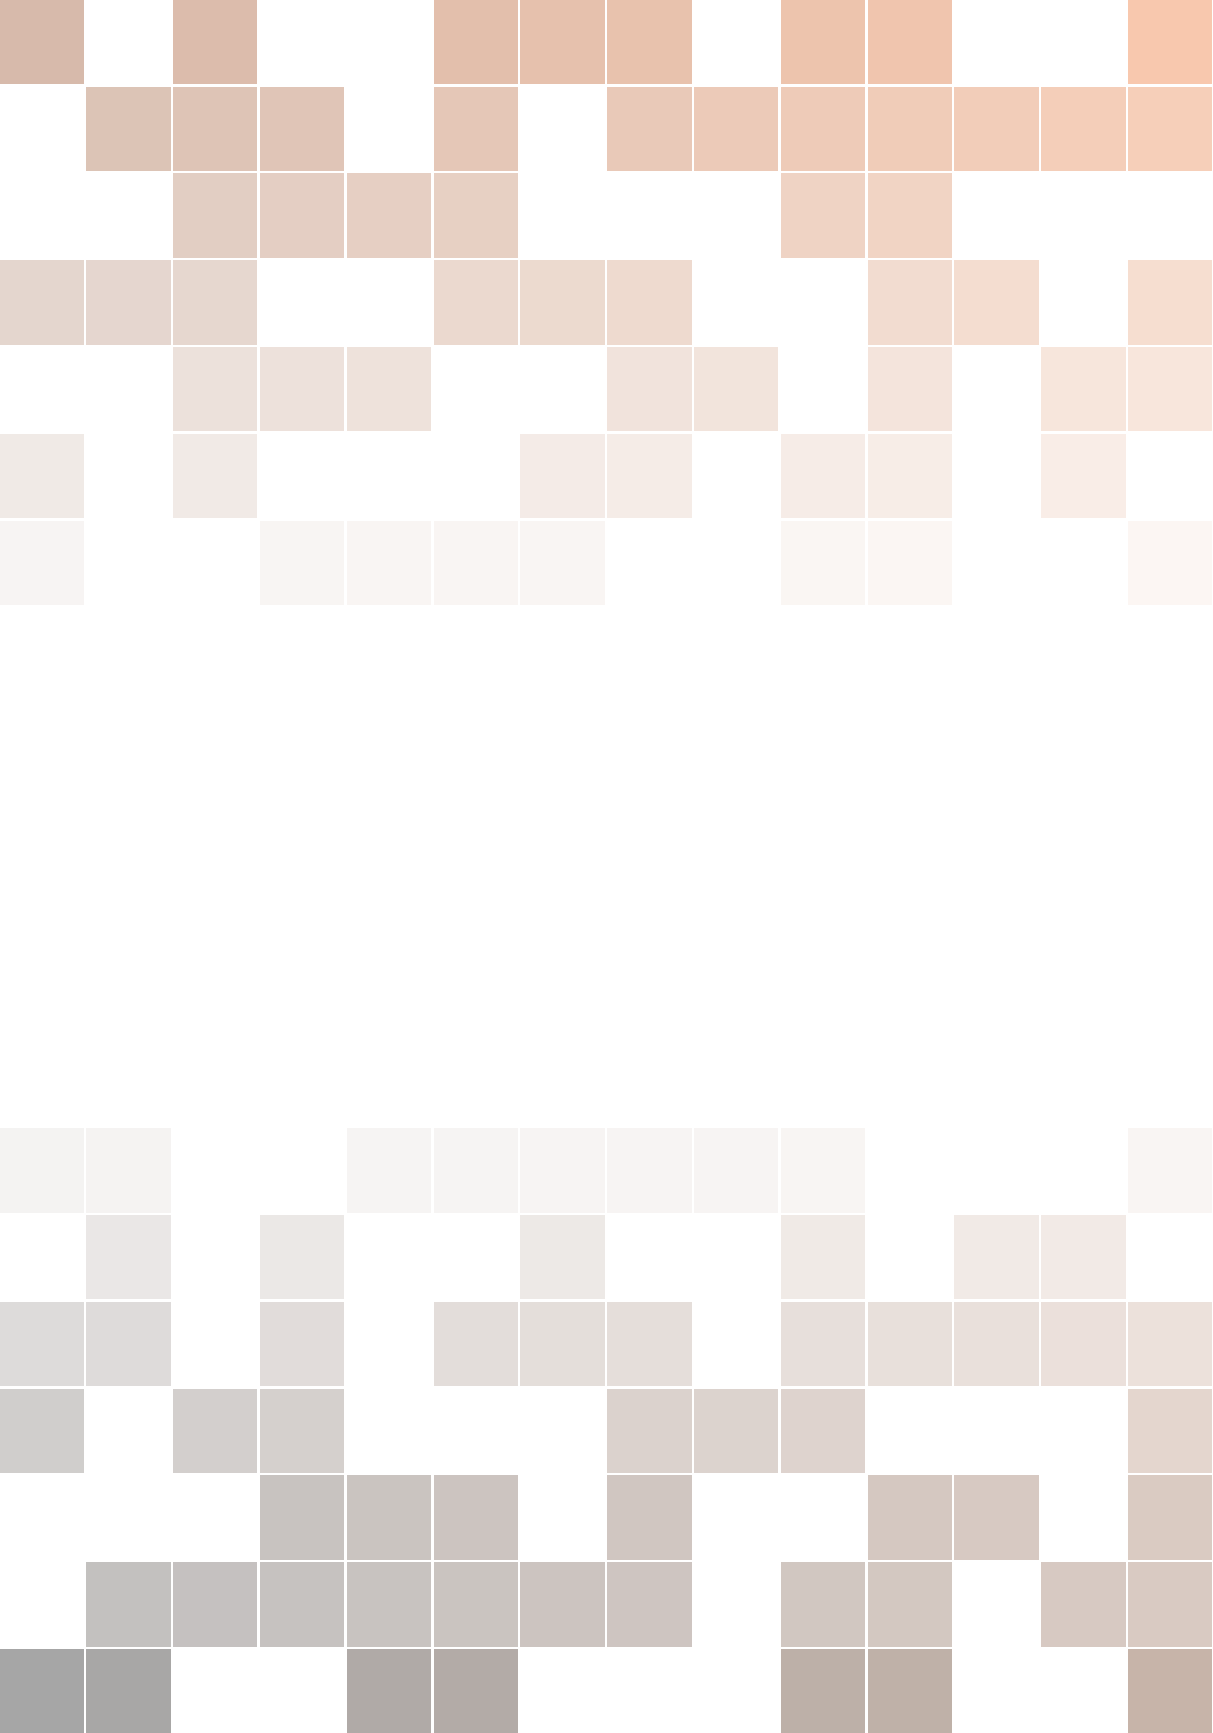
\includegraphics[width=\paperwidth]{background}};
\draw (current page.center) node [fill=ocre!30!white,fill opacity=0.6,text opacity=1,inner sep=1cm]{\Huge\centering\bfseries\sffamily\parbox[c][][t]{\paperwidth}{\centering Informatique\\[15pt] % Book title
{\Large Travaux Pratiques}\\[20pt] % Subtitle
{\huge Axel LE BOT}}}; % Author name
\end{tikzpicture}
\vfill
\endgroup

%----------------------------------------------------------------------------------------
%	COPYRIGHT PAGE
%----------------------------------------------------------------------------------------

\newpage
~\vfill
\thispagestyle{empty}

\noindent Copyright \copyright\ 2017-2018 Axel LE BOT \\ % Copyright notice

\noindent Licensed under the Creative Commons Attribution-NonCommercial 3.0 Unported License (the ``License''). You may not use this file except in compliance with the License. You may obtain a copy of the License at \url{http://creativecommons.org/licenses/by-nc/3.0}. Unless required by applicable law or agreed to in writing, software distributed under the License is distributed on an \textsc{``as is'' basis, without warranties or conditions of any kind}, either express or implied. See the License for the specific language governing permissions and limitations under the License.\\ % License information

%----------------------------------------------------------------------------------------
%	TABLE OF CONTENTS
%----------------------------------------------------------------------------------------

%\usechapterimagefalse % If you don't want to include a chapter image, use this to toggle images off - it can be enabled later with \usechapterimagetrue

\chapterimage{cover_table_of_contents} % Table of contents heading image

\pagestyle{empty} % No headers

\tableofcontents % Print the table of contents itself

\cleardoublepage % Forces the first chapter to start on an odd page so it's on the right

\pagestyle{fancy} % Print headers again

%----------------------------------------------------------------------------------------
%	PART ONE
%----------------------------------------------------------------------------------------

\part{Shell}

\chapterimage{./shell/unix} % Chapter heading image
\chapter{Shell - TP1 : Manipulations de l’environnement et des fichiers sous UNIX}
    \section{Exercice 1 : Découverte de quelques commandes d'archivage}
    \textit{L'objectif de cet exercice est de découvrir et manipuler les commandes de téléchargement, d'archivage, de compression et de décompression de fichier}
        \subsection{1. Récupération et décompression d'une archive}
            La commande \texttt{wget https://cloud.infotro.fr/ITC313/archive.tar} permet de télécharger l'archive présent à cette adresse.
            \begin{itemize}
                \item L'option \texttt{-x} permet de restaurer les fichiers contenus dans une archive.
                \item L'option \texttt{-c} permet de créer une nouvelle archive.
                \item L'option \texttt{-f} permet d'utilise le fichier archive F ou le périphérique F (par défaut /dev/rmt0).
            \end{itemize}
            9 fichiers était présent dans cette archive
        \subsection{2. Manipulation de fichiers}
            \texttt{file .\/*}
            Afin de renommer le fichier j'utilise cette commande \texttt{mv image4.jpg image4.jpg2}.
            Le fichier \texttt{script.txt} fait 170Ko.
            La commande \texttt{gzip} sur \texttt{script.txt} a compressé le fichier.
            Le fichier fait maintenant  65Ko.
            La compréssion est donc d'environ 38.235\%.
            Après décompression avec la commande \texttt{gunzip} le fichier fait maintenant 170Ko, qui est la taille initial du fichier.
        \subsection{3. Création d'une nouvelle archive}
            La nouvelle archive fait 850Ko soit 1Ko de moins que l'ancienne archive. Surement à cause du nom de fichier jp2 changé.
            La somme des tailles des fichiers dans l'archive est égale à 845479 soit 845Ko, on observe une différence de 5Ko.
            La compression de l'archive (créé précédemment) fait 617Ko soit une différence de 228Ko.
            L'option \texttt{-z} utilise gzip pour comprésser l'archive.
            Elle revient totalement à créé une archive puis la compresser puisque d'après les test la taille n'est pas différente.
            La Commande \texttt{tar -c -z *.jpg *.txt *.jp2} devrait normalement afficher dans le terminal le résultat.
            La Commande \texttt{tar -c -z *.jpg *.txt *.jp2 > nouvelleArchive3.tar.gz} redirige bien le résultat dans un fichier.
            La redirection du flux dans un fichier recréer une archive compréssé similaire à la deuxième créé.
            En conclusion l'archive 2 et 3 donne le même résultat et sont plus petit que l'archive 1 puisqu'elles sont compréssés.
    \section{Exercice 2 : Utilisation des masques de création de fichiers}
        \subsection{1.}
            \begin{minted}[linenos,
                            frame=lines]{bash}
                $ touch Raphael.txt
                $ umask 0666
                $ touch Donatello.txt
                $ umask 0331
                $ touch Michelangelo.txt
                $ umask 0661
                $ touch Leonardo.txt
                $ umask 0000
            \end{minted}
        \subsection{2. et 3.}
            Il n'est pas possible de créer de donner plus de droit que la limitation par défaut du systeme.
            ( application umask par défaut 666 sur fichier et 777 sur repertoire)
    \section{Exercice 3 : Manipulation du Systeme de fichier et des droits de navigation}
        \subsection{1.}
            L'archive contient 5 images.
        \subsection{3.}
            \texttt{/home/ESIREM-AD/al669724/Documents/Shell/TPs/TP1/Ex3/images/Chinpokomon/P-Z/Vamporc.png}
        \subsection{4.}
            \texttt{../P-Z/Vamporc.png}
        \subsection{6.}
            L'option \texttt{-z} permet de compresser l'archive.
            \begin{verbatim}
                $ tar -xczf ITC313_TP_Shell_lebot.axel.tar.gz
            \end{verbatim}
            permettra de décompresser et extraire l'archive.
        \subsection{7.}
            Toutes les permissions sont conservés.
    \section{Exercice 4 : Manipulation d'expression régulière}
        \subsection{2.}
            Les lignes contenant la suite de lettres "ette".
        \subsection{3.}
            Les lignes contenant la lettre "T".
        \subsection{4.}
            Les lignes commencant par la lettre "T".
        \subsection{5.}
            \texttt{\^} signifie "début".
        \subsection{6.}
            Les lignes finissant par "te".
        \subsection{7.}
            Les lignes contenant la suite de caractère "c", un caractère, "r".
        \subsection{8.}
            Les lignes contenant "oui" ou "non".
        \subsection{9.}
            \begin{itemize}
                \item '\$' -> en fin
                \item '|' -> ou
                \item '.' -> un caractère
            \end{itemize}
        \subsection{10.}
            Permet d'afficher uniauement la partie correspondant à la recherche.
        \subsection{11.}
           Une suite de 4 lettre Majuscule.
        \subsection{12.}
            Une suite d'au moins une Majuscule et un minuscule
        \subsection{13.}
            Les mots commencant par une majuscule aisni que les lettre majuscules.
        \subsection{15.}
            Permet de récupérer les addresse e-mail.
        \subsection{16.}
            Permet de récupérer les numéro de téléphone.
        \subsection{17.}
            ((bien))((joue))((tu))((as))((trouve))((la))((reponse))((a))((la))((derniere))((question))

\chapterimage{./shell/writing} % Chapter heading image
\chapter{Shell - TP2 : Scripts Shell}
    \section{Exercice 5 : Un premier script}
        \lstinputlisting[language=Bash]{../sources/shell/TP2/ex5.sh}
    \section{Exercice 6 : Comptage des paramètres}
        \lstinputlisting[language=Bash]{../sources/shell/TP2/ex6-parametres.sh}
        \lstinputlisting[language=Bash]{../sources/shell/TP2/ex6-parametres2.sh}
    \section{Exercice 7 : Portée des variables}
        \paragraph{1. Portée des variables locales}
            La variable créé dans le terminal n'est pas accessible depuis un script.
        \paragraph{2. Portée limitée au shell}
            Les variables sont local au terminal
        \paragraph{3. Étendre la portée de la valeur d’une variable locale}


%----------------------------------------------------------------------------------------
%	PART TWO
%----------------------------------------------------------------------------------------

\part{C++}

\chapterimage{./cpp/cover1.png} % Chapter heading image
\chapter{TP1+TP2 : Exercices sur les tableaux et matrices, et Fonctions récursives}
    \section{Exercice sur des tableaux}
        \subsection{Fonction sur les tableaux non triés}
            \subsubsection{Exercice 1 : Algorithmes de parcours classiaues sur tableau non triés}
	              Quelques copier coller ont suffit.
                Les tests ont bien été éffectué.
            \subsubsection{Exercice 2 : Ajout et suppression d'éléments tableaux non triés}
        \subsection{Algorithmes de tri de tableaux}
            \subsubsection{Exercice 3 : Trier des tableaux aléatoires}
        \subsection{Fonctions sur les tableaux triés}
            \subsubsection{Exercice 4 : Algorithmes de parcours classiques sur tableau non triés}
            \subsubsection{Exercice 5 : Ajout et suppression d’éléments sur tableaux triés}
        \subsection{Exercice sur les Fonctions récursives}
  	    \subsubsection{Exercice 6 : Definition de fonction recursive}
  	    \subsubsection{Exercice 7 : Algorithme recursif sur matrice}

\chapterimage{./cpp/cover1.png} % Chapter heading image
\chapter{TP3 + TP4 : manipulation des arbres}
    \section{Algorithmes sur arborescences binaires de recherche (ABR) non équilibrées}
        \subsection{Exercice 1 : Mise en place d’ABR et premiers algorithmes}
        \subsection{Exercice 2 : Algorithmes récursifs sur arborescences}
    \section{Modification et parcours d’ABR non équilibrées}
        \subsection{Exercice 3 : Insertion et suppression de valeurs dans une arborescence}
    \section{Parcours d’arborescences binaires}
        \subsection{Exercice 4 : Parcours sur arbres}

\chapterimage{./Pictures/cover-gear} % Chapter heading image
\chapter{TP5+TP6 : Hiérarchie de processus, signaux}
\textit{Dans ce TP, nous allons revenir sur quelques commandes en shell pour illustrer le fonctionnement de manière simple, puis nous déporterons ces concepts au travers d’appels systèmes dans une fonction C.}

\section{Gestion des signaux : envoi et reception}
\textit{Les exercices de cette question se concentrent sur les mécanismes d’envoi et de reception des signaux. Ils visent prioritairement à comprendre comment on envoie un signal, quelles sont les conditions nécessaires pour qu’un processus accepte de recevoir un signal, et comment dérouter l’exécution normale d’un programme lorsque ce dernier reçoit un signal. Nous montrons notamment que le concept d’envoi et réception de signaux s’applique aussi bien pour des scripts shell que pour des programmes écrits dans un langage de programmation, ici le C. Dans la section d’après, nous verrons comment ces signaux sont utilisés pour gérer les processus, notamment les phases d’exécution et d’arrêt prématuré.}

\subsection{Exercice 1 : Droits et signaux}
\textit{Cet exercice à pour objectif de nous faire comprendre la nation de droits associés aux signaux. Pour cela, nous utiliserons plusieurs commandes shell, notamment la commande \mintinline{shell}{ps} qui permet de lister les processus actifs sur une machine, et la commande \mintinline{shell}{kill} qui permet d’envoyer un signal à un processus identifié par son pid.}

La commande \mintinline{shell}{kill -l} nous permet de lister l'ensemble des signaux. Pour pouvoir les compter nous éxecutons la commande \mintinline{shell}{kill -l | wc -w} qui compte 31 signaux sur ma machine. On peut envoyer un signal à un processus dont on connait son \texttt{PID} à l'aide de la commande \mintinline{shell}{kill -<SIG_NAME> <PID>}. Par exempler nous pouvons tuer le processus 1285 à l'aide de la commande \mintinline{shell}{kill -SIGKILL 1285}.

Nous écrivons un programme permettant de boucler à l'infinie à l'aide d'une boucle \mintinline{cpp}{while(1)}. Le programme était en \texttt{BASH} je l'ai implémenté en C :
\inputminted[linenos,firstline=8,lastline=14]{cpp}{../sources/cpp/TP5-6/ex1.c}

En éxecutans ce programme dans et en récupérant son PID, nous pouvons dans un terminal, en utilisant la commande \mintinline{shell}{kill} envoyer un signal SIGKILL à ce processus et ainsi mettre fin au programme en le tuant. Si j'envoie le signal à un processus dont je ne suis pas le propriétaire ( appartenant à autre utilisateur ou au root), l'erreur "Operation not authorized" s'affiche. Je peut le vérifier en éxécutant la commande sur un processus root et en vérificant son éxécution dans la liste des processus à l'aide de la commande \mintinline{shell}{top}.

\subsection{Exercice 2 : capture de signal et traduction en langage C}
\textit{Cet exercice nous apprendra capturer des signaux, c’est à dire que l’on peut détecter la réception d’un signal envoyé par un autre processus, et redéfinir le comportement à adopter, c’est à dire la suite d’instructions à exécuter, lorsqu’un signal est détecté.}

J'ai écrit un script shell comportant une boucle infinie affichant un "." chqaue seconde. Le script capture aussi le signal \texttt{SIGINT} et \texttt{SIGUSR1} ainsi si l'utilisateur appuie sur \texttt{CTRL+C} ou envoie un signal \texttt{SIGUSR1} pendant son éxécution un message sera affiché. Ce script lancé ne pourra donc pas être arrété si l'utilisateur appuie sur \texttt{CTRL+C} ou utilise la commande \mintinline{shell}{killl -SIGKILL <PID>}.
Le script et le suivant :
\inputminted{bash}{../sources/cpp/TP5-6/ex2-boucle.sh}
Et maintenant en langage \texttt{C} :
\inputminted[linenos,firstline=10,lastline=32]{cpp}{../sources/cpp/TP5-6/ex2.c}

\subsection{Exercice 3 : Capture de signaux et redirections (exercice difficile)}
\textit{Cet exercice permet de capturés des signaux et les redirigés, c’est à dire que lorsque le signal est reçu, on redéfinit le comportement par défaut qu’aurait du avoir le processus. Dans un premier temps, nous allons voir quel est le comportement par défaut des processus lors de la réception d’un signal. Dans un  second temps, nous allons redéfinir le comportement d’un processus à la réception d’un signal.}

Plusieurs signaux permettent de terminer l'exécution d'un processus. Afin de pouvoir savoir lesquels nous allons écrire un script. Pour chaque signal X, un processus sera lancé en arrière plan, ici le script de la boucle infinie sera utilisé. Son PID sera retrouvé grace à la variable \mintinline{bash}{$!} afin de lui envoyer le signal X. À l'aide de la commande \mintinline{shell}{ps -p <PID>} nous saurons si le processus à été arrété, ainsi on pourra conclure que le signal X tuje ou pas le processus.
Voici le script :
\inputminted[linenos]{bash}{../sources/cpp/TP5-6/ex3-testKillerSignal.sh}

\subsection{Exercice 4 : envoi multiples et capture de signal en C}
\textit{Au terme des exercices précédents nous avons compris les notions de signal, de redirection et de mise en oeuvre en langage shell. L'objectif de cet exercice est la simple traduction de ce qui a été vu en shell en langage C, et l’étude d’une autre commande nommée killall}
Nous avons besoin dans un premier temps du code ayant une boucle infinie et capturant le signal SIGINT (CTRL+C). Le script est ci-dessous :
\inputminted{bash}{../sources/cpp/TP5-6/ex4-captureShell.sh}
Et maintenant en langage \texttt{C} :
\inputminted[linenos,firstline=10, lastline=28]{cpp}{../sources/cpp/TP5-6/ex4.c}
Nous pouvons maintenant lancer 3 processus de notre programme C afin de les tuers avec la commande \mintinline{shell}{killall -SIGINT ex4}.
On essaie aussi de les mettre en pause et des les relancer grace aux commandes
\begin{itemize}
\item \mintinline{shell}{killall -SIGSTOP ex4}
\item \mintinline{shell}{killall -SIGCONT ex4}
\end{itemize}
Puis nous les tuons grace à la commande \mintinline{shell}{killall -9 ex4}

\section{Gestion des processus}

\subsection{Exercice 5 : Processus en premier-plan / Arriere-plan}
\textit{Nous allons voir ici comment manipuler les processus pour les passer tantôt en premier-plan, tantôt en arrière-plan, les stopper et les relancer. Ces manipulations sont rendues possibles par l’utilisation de signaux, et les fonctionnalités de deux programmes : bg (background) et fg (foreground)}
La commande \mintinline{shell}{ps aux} permet d'afficher l'etat d'execution des processus.
Il affiche le status du processus :
\begin{itemize}
\item R : "runnable", veut dire que le processus est prêt à être éxécuté.
\item S : "sleeping", veut dire que le processus est endormi.
\item D : veut dire que le processus est sommeil interruptible.
\item T : "traced", veut dire que le processus est arrété ou suivi.
\item Z : zombie
\end{itemize}
Le \texttt{+} qui suit indique si le processus est en arrière plan.

\subsection{Exercice 6 : Duplication et recouvrement de processus}
\textit{Dans cet exercice, nous recouvrons un processus existant, d’abord au travers d’un script shell, puis en appliquant ce concept au sein d’un programme C.}
\paragraph{1. Manipulation de la commande \mintinline{shell}{exec} sur un shell}
\begin{itemize}
  \item La commande \mintinline{shell}{exec} Permet d'executer un programme. ( couplé a \mintinline{bash}{fork} )
  \item La commande \mintinline{bash}{sleep 3} permet d'attendre 3 secondes.
  Utiliser dans un terminal, le terminal se fermera apr`s son exécution.
\end{itemize}

\paragraph{2. Application dans un script shell}
\begin{minted}
exec echo "Bonjour";
exec echo "bonsoir";
\end{minted}
À exécution du script ci-dessus uniquement "Bonjour" s'affichera dans le terminal. On peut ainsi constater qu'après l'utilisation de la commande mintinline{shell}{exec}, le programme se termine.

\paragraph{3. Application dans un programme C}
\textit{Dans cette partie nous verrons comment lancer  des programmes depuis un programme.}

Le programme implémenté ci-dessous permet deux choisir deux tache :
\beging{itemize}
\item Si vous entrez \texttt{1} le processus sera remplacer avec le programme \texttt{/bin/hostname}.
\item Si vous entrez \texttt{2} le processus sera remplacer avec le programme \texttt{/bin/date}.
\end{itemize}

\inputminted[linenos,firstline=8, lastline=23]{cpp}{../sources/cpp/TP5-6/ex6.c}

\section{Gestion des processus - Suite}
\subsection{Exercice 7 : Duplication de processus}
\textit{L’objectif de cet exercice est de comprendre la notion de processus parent et de processus enfant lors de la duplication d’un processus par l’appel à la fonction \mintinline{shell}{fork()}. Nous y revoyons la notion de PID et PPID (ou PID du parent) vus en cours. L’objectif est de mettre en évidence le role de l’appel à l’instruction fork() ainsi que la particularité de son code retour, et d’identifier que lors d’une duplication, le processus nouvellement créé ne reprend pas au début de son code mais poursuit l’exécution du processus parent. On rappelle que \mintinline{shell}{fork()} retourne 0 dans le processus nouvellement créé (fils) et une valeur strictement supérieure à 0 sinon (qui correspond au PID du processus nouvellement créé)}

Dans ce programme nous devons faire en sorte que le programme principale se duplique avec la commande fork() et que nous puissions identifier les enfants et parent en écrivant dans la console son rôle, son PID et le PID père.

\inputminted[linenos,firstline=9, lastline=27]{cpp}{../sources/cpp/TP5-6/ex7-fork1.c}

Dans ce programme nous devons faire en sorte que le programme principale se duplique avec la commande fork(), que l'enfant se duplique à son tour et que chaque processus puisse être identifier comme enfants, parent ou grand-parent en écrivant dans la console son rôle, son PID et le PID père.

\inputminted[linenos,firstline=9, lastline=30]{cpp}{../sources/cpp/TP5-6/ex7-fork2.c}

\subsection{Exercice 8 : Creation et destruction de processus}
\textit{Cet exercice rappelle les notions de processus zombie et processus orphelin, et définit les modalités d’apparition de ces deux types particuliers de processus.}
En lançant la commande \mintinline{shell}{ps -aux} on peut observer le statut des processus.

\paragraph{1. Processus zombie}
Un processus zombie est un processus présent alors que sont processus parent ayant terminé son exécution, il reste présent sur le système, en attente d'être pris en compte par son processus parent..
Pour créer un processus zombie nous pouvons dans le processus père ometre d'utiliser la fonction \mintinline{cpp}{wait()}.

\paragraph{2. Processus orphelin}
Un processus orphelin est un processus présent alors que sont processus parent est mort. Le processus orphelin est donc "adopté" par le processus 1, le processus "init"
Pour créer un processus orphelin nous pouvons dans le processus enfant (\mintinline{cpp}{fork()==0}) executer la commande \mintinline{cpp}{sleep(60)} afin d'endormir le processus 60 secondes et le processus père \mintinline{cpp}{fork!=0} pourrais executer la commande (\mintinline{cpp}{exit(0)}) afin de terminer son execution.

\subsection{Exercice 9 : Evaluation du nombre de processus}
\textit{L’objectif de cet exercice est de comprendre le résultat de l’appel à l’instruction \mintinline{shell}{fork()} ainsi que la particularité de son code retour, et d’identifier que lors d’une duplication, le processus nouvellement créé ne reprend pas au début de son code mais poursuit l’exécution du processus parent. On rappelle que \mintinline{cpp}{fork()} retourne 0 dans le processus nouvellement créé (fils) et une valeur strictement supérieure à 0 sinon (qui correspond au PID du processus nouvellement créé).}

\paragraph{1. premier programme :}
\inputminted[linenos,firstline=7, lastline=11]{cpp}{../sources/cpp/TP5-6/ex9-programme1.c}
Nous pouvons expliquer le code ci-dessus par le schema suivant :
\begin{figure}[H]
\centering
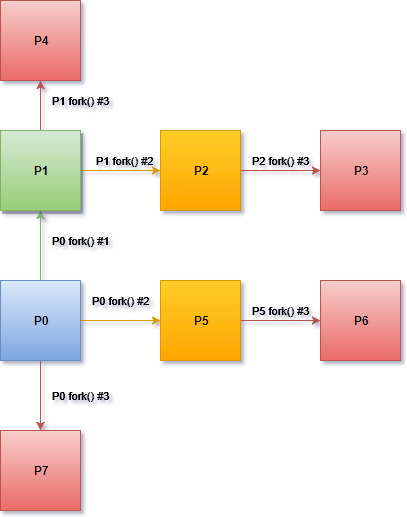
\includegraphics[width=200pt]{./cpp/Pictures/tp5+tp6-ex9-programme1}
\caption{Duplication de processus 1}
\label{Duplication de processus 1}
\end{figure}

\paragraph{2. deuxième programme :}
\inputminted[linenos,firstline=7, lastline=11]{cpp}{../sources/cpp/TP5-6/ex9-programme2.c}
Nous pouvons expliquer le code ci-dessus par le schema suivant :
\begin{figure}[H]
\centering
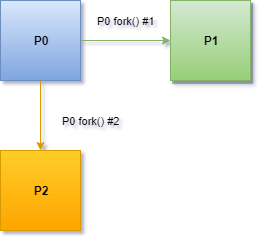
\includegraphics[width=200pt]{./cpp/Pictures/tp5+tp6-ex9-programme2}
\caption{Duplication de processus 2}
\label{Duplication de processus 2}
\end{figure}

\paragraph{3. troisieme programme :}
\inputminted[linenos,firstline=7, lastline=15]{cpp}{../sources/cpp/TP5-6/ex9-programme3.c}
Nous pouvons expliquer le code ci-dessus par le schema suivant :
\begin{figure}[H]
\centering
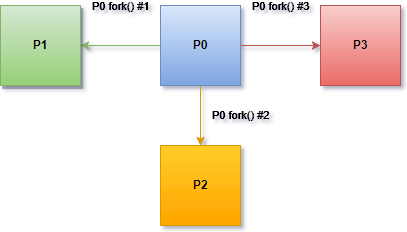
\includegraphics[width=200pt]{./cpp/Pictures/tp5+tp6-ex9-programme3}
\caption{Duplication de processus 3}
\label{Duplication de processus 3}
\end{figure}

\subsection{Exercice 10 : Conjonctions, Disjonctions, et Duplication}
\textit{L’objectif de cet exercice est de comprendre le résultat de l’appel à l’instruction \mintinline{cpp}{fork()} ainsi que la particularité de son code retour, et d’identifier que lors d’une duplication, le processus nouvellement créé ne reprend pas au début de son code mais poursuit l’exécution du processus parent.}

En éxécutant quelques programmes exemple ci-dessous nous pouvons déterminer le fonctionnement des conjonctions et des disjonctions.

\paragraph{1. premier programme :}
\inputminted[linenos,firstline=8, lastline=11]{cpp}{../sources/cpp/TP5-6/ex10-conjonction1.c}
\begin{enumerate}
\item Le processus père P0 : éxécute le premer \mintinline{cpp}{fork()} créant le processus P1 et retourne une valeur non-nulle et s'arrete.
\item Le processus fils P1 : la valeur du premier \mintinline{cpp}{fork()} est égale à 0 et évalue \mintinline{cpp}{&&}
\item Le processus fils P1 : éxécute donc le deuxième \mintinline{cpp}{fork()} fork créant P2 ainsi que le troisieme \mintinline{cpp}{fork()} créant P3
\item Le processus fils P2 : la valeur du deuxième \mintinline{cpp}{fork()} retourne 0, cour-circuite \mintinline{cpp}{&&} et s'arrete.
\item Le processus fils P3 : la valeur du troisième \mintinline{cpp}{fork()} retourne 0 et s'arrete.
\end{enumerate}

Nous pouvons expliquer le code ci-dessus par le schema suivant :
\begin{figure}[H]
\centering
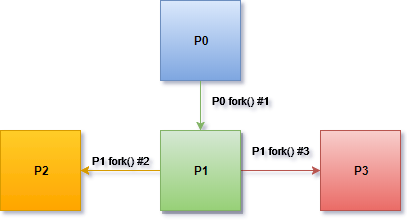
\includegraphics[width=200pt]{./cpp/Pictures/tp5+tp6-ex10-conjonction1}
\caption{Conjonction de processus 1}
\label{Conjonction de processus 1}
\end{figure}

\paragraph{2. deuxième programme :}
\inputminted[linenos,firstline=8, lastline=11]{cpp}{../sources/cpp/TP5-6/ex10-conjonction2.c}
\begin{enumerate}
\item Le processus père P0 éxécute le premier \mintinline{cpp}{fork()} créant le processus P1 et retourne une valeur non-nulle.
\item Le processus fils P1 la valeur du premier \mintinline{cpp}{fork()} est égale à 0 et court-circuite \mintinline{cpp}{&&} et s'arrete.
\item Le processus père P0 : la valeur du premier \mintinline{cpp}{fork()} est non-nulle et évalue \mintinline{cpp}{||} et effectue le deuxième \mintinline{cpp}{fork}.
\item Le processus fils P2 : la valeur du deuxième \mintinline{cpp}{fork()} retourne 0 et exécute donc le troisieme \mintinline{cpp}{fork()} créant P3.
\item Le processus fils P2 s'arrete.
\item Le processus fils P3 s'arrete.
\end{enumerate}
Nous pouvons expliquer le code ci-dessus par le schema suivant :
\begin{figure}[H]
\centering
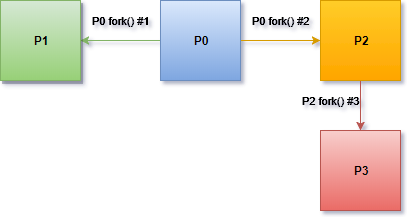
\includegraphics[width=200pt]{./cpp/Pictures/tp5+tp6-ex10-conjonction2}
\caption{Conjonction de processus 2}
\label{Conjonction de processus 2}
\end{figure}

\subsection{Exercice 11 : Terminaison normale de processus}
\textit{L’objectif de cet exercice est de placer correctement les instructions \mintinline{cpp}{wait()}}

Lorsque le processus fils se termine avant le processus père, il devient un zombie. Pour permettre à un processus fils en état zombie de disparaître complètement, on utilise la \mintinline{cpp}{wait()}.

\paragraph{1. premier programme :}
\inputminted[linenos,firstline=8, lastline=14]{cpp}{../sources/cpp/TP5-6/ex11-programme1.c}

\paragraph{2. deuxième programme :}
\inputminted[linenos,firstline=8, lastline=17]{cpp}{../sources/cpp/TP5-6/ex11-programme2.c}

\paragraph{3. troisieme programme :}
\inputminted[linenos,firstline=8, lastline=22]{cpp}{../sources/cpp/TP5-6/ex11-programme3.c}

\chapter{TP7 + TP8 programmation : communication socket}
    \section{Communication distante en utilisant l’outil netcat}
        \subsection{Exercice 1 : Découverte de la commande nc : netcat}
        \subsection{Exercice 2 : Utilisation de la commande nc : netcat pour le transfert de fichier et l’évaluation de
la bande passante}
        \subsection{Exercice 3 : Une histoire de serveurs concurrents ...}
        \subsection{Exercice 4 : Comprendre une requête HTTP}
    \section{Développement d’un client et d’un serveur en C}
        \subsection{Exercice 5 : Mise en place d’une communication en mode non connecte}
        \subsection{Exercice 6 : Création d’une architecture (client UDP) - (relai UDP-TCP)- (serveur TCP)}
    \section{Exercices bonus}
        \subsection{Exercice 7 : Résolution de noms}
        \subsection{Exercice 8 : Serveur multi-client en mode connecte}

\chapterimage{./cpp/cpp} % Chapter heading image
\chapter{TP9+TP10 : Héritage multiple et modélisation}
        \section{Exercice 1 : Organisation d’un jeu de combat au tour par tour}

\chapter{TP11 + TP12 Projet de synthèse}
        \section{Realisation d’un jeu de Puissance 4}


%----------------------------------------------------------------------------------------

\part{Autres}

\section{Figure}\index{Figure}

\begin{figure}[h]
\centering
\includegraphics[scale=0.5]{placeholder}
\caption{Figure caption}
\end{figure}

%----------------------------------------------------------------------------------------
%	BIBLIOGRAPHY
%----------------------------------------------------------------------------------------

\chapter*{Bibliography}
\addcontentsline{toc}{chapter}{\textcolor{ocre}{Bibliography}}
\section*{Books}
\addcontentsline{toc}{section}{Books}
\printbibliography[heading=bibempty,type=book]
\section*{Articles}
\addcontentsline{toc}{section}{Articles}
\printbibliography[heading=bibempty,type=article]

%----------------------------------------------------------------------------------------
%	INDEX
%----------------------------------------------------------------------------------------

\cleardoublepage
\phantomsection
\setlength{\columnsep}{0.75cm}
\addcontentsline{toc}{chapter}{\textcolor{ocre}{Index}}
\printindex

%----------------------------------------------------------------------------------------

\end{document}
